\documentclass{article}

\usepackage{indentfirst}
\usepackage{graphicx}
\usepackage{subfigure}

\begin{document}

\setlength{\parindent}{2em}
\linespread{1}

\title{Project Report : Grabcut}
\author{Zeyuan Shang \\ 2011012032 \\ Tsinghua University}
\date{\today}
\maketitle

\section{Introduction}
    
    The problem of efficient, interactive foreground/background segmentation in still images is of great practical importance in image editing. The resulting foreground object is an alpha-matte which reflects the proportion of foreground and background.

    In this project, we experimentally examined approach proposed in \cite{Rother}, which could  extract a foreground object.

\section{Aproach}

    \subsection{Image segmentation by graph cut}

        An energy function E is defined so that its minimum should correspond to a good segmentation. This is captured by a “Gibbs” energy of the form:
        
        $$E(\alpha, \theta, z) = U(\alpha, \theta, z) + V(\alpha, z)$$

        The data term $U$ evaluates the fit of the opacity distribution $\alpha$ to the data $z$, given the histogram model $\theta$, and is defined to be:

        $$U(\alpha, \theta, z) = \sum_{\pi} -\log{h(z_{n};\alpha_{n})}$$

        The smoothness term can be written as:

        $$V(\alpha, z) = \gamma \sum_{(m, n) \in C} dis(m, n)^{-1} [\alpha_{n} \not=] e^{-\beta (z_{n} - z_{m})^{2}}$$

        The constant $\beta$ is chosen to be:

        $$\beta = \frac{1}{2 (z_{n} - z_{m})^{2}}$$

    \subsection{Gaussian Mixture Model}

        As we know, the Gaussian Mixture Model is as follows:

        $$D(x) = \sum_{i = 1}^{K}(\pi_{i} g_{i}(x; \mu_{i}, \Sigma_{i})), \sum_{i = 1}{K}(\pi_{i} = 1), 0 <= \pi_{i} <= 1$$

        $$g(x; \mu, \Sigma) = \frac{1}{\sqrt{(2\pi)^{d} |\Sigma|}} e^{-\frac{1}{2} (x - \mu)^{T} \Sigma^{-1} (x - \mu)}$$

    \subsection{Colour Data Modelling}

        From 2.1 and 2.2, we could get:

        $$D(\alpha_{n}, k_{n}, \theta, z_{n}) = -\log(\pi(\alpha_{n}, k_{n})) + \frac{1}{2} \log(det \Sigma(\alpha_{n}, k_{n})) + \frac{1}{2} [z_{n} - \mu (\alpha_{n} - k_{n})]^{T} \Sigma(\alpha_{n}, k_{n})^{-1} [z_{n} - \mu (\alpha_{n} - k_{n})]$$

    \subsection{Segmentation by Iterative Energy Minimization}

        \subsubsection{Initialize}

            \begin{itemize}
                \item User initialises trimap T by supplying only $T_{B}$. The foreground is set to $T_{F} = /0$; $T_{U} = T_{B}$, complement of the background.
                \item Initialise $\alpha_{n} = 0$ for $n \in T_{B}$ and $\alpha_{n} = 1$ for $n \in T_{U}$
                \item Background and foreground GMMs initialised from sets $\alpha_{n} = 0$ and $\alpha_{n} = 1$ respectively
            \end{itemize}

        \subsubsection{Iterative minimisation}

            \begin{itemize}
                \item Assign GMM components to pixels: for each n in $T_{U}$,
                        $$k_{n} := arg \min_{k_{n}} D_{n}(\alpha_{n}, k_{n}, \theta, z_{n})$$.
                \item Learn GMM parameters from data z:
                        $$\theta := arg \min_{\theta} U(\alpha, k, \theta, z)$$.
                \item Estimate segmentation: use min cut to solve:
                        $$\min_{\alpha_{n} : n \in T_{U}} \min_{k} E(\alpha, k, \theta, z)$$.
                \item Repeat from step 1, until convergence.
            \end{itemize}

\section{Result}

    Besides the output of the Grabcut, I also made some comparsion with the GrabCut in OpenCV, and my implementation is about $10-20\%$ faster than OpenCV on my computer. Please see figures below to check the results.

    \begin{figure}
        \begin{center}
            \subfigure[input]{
                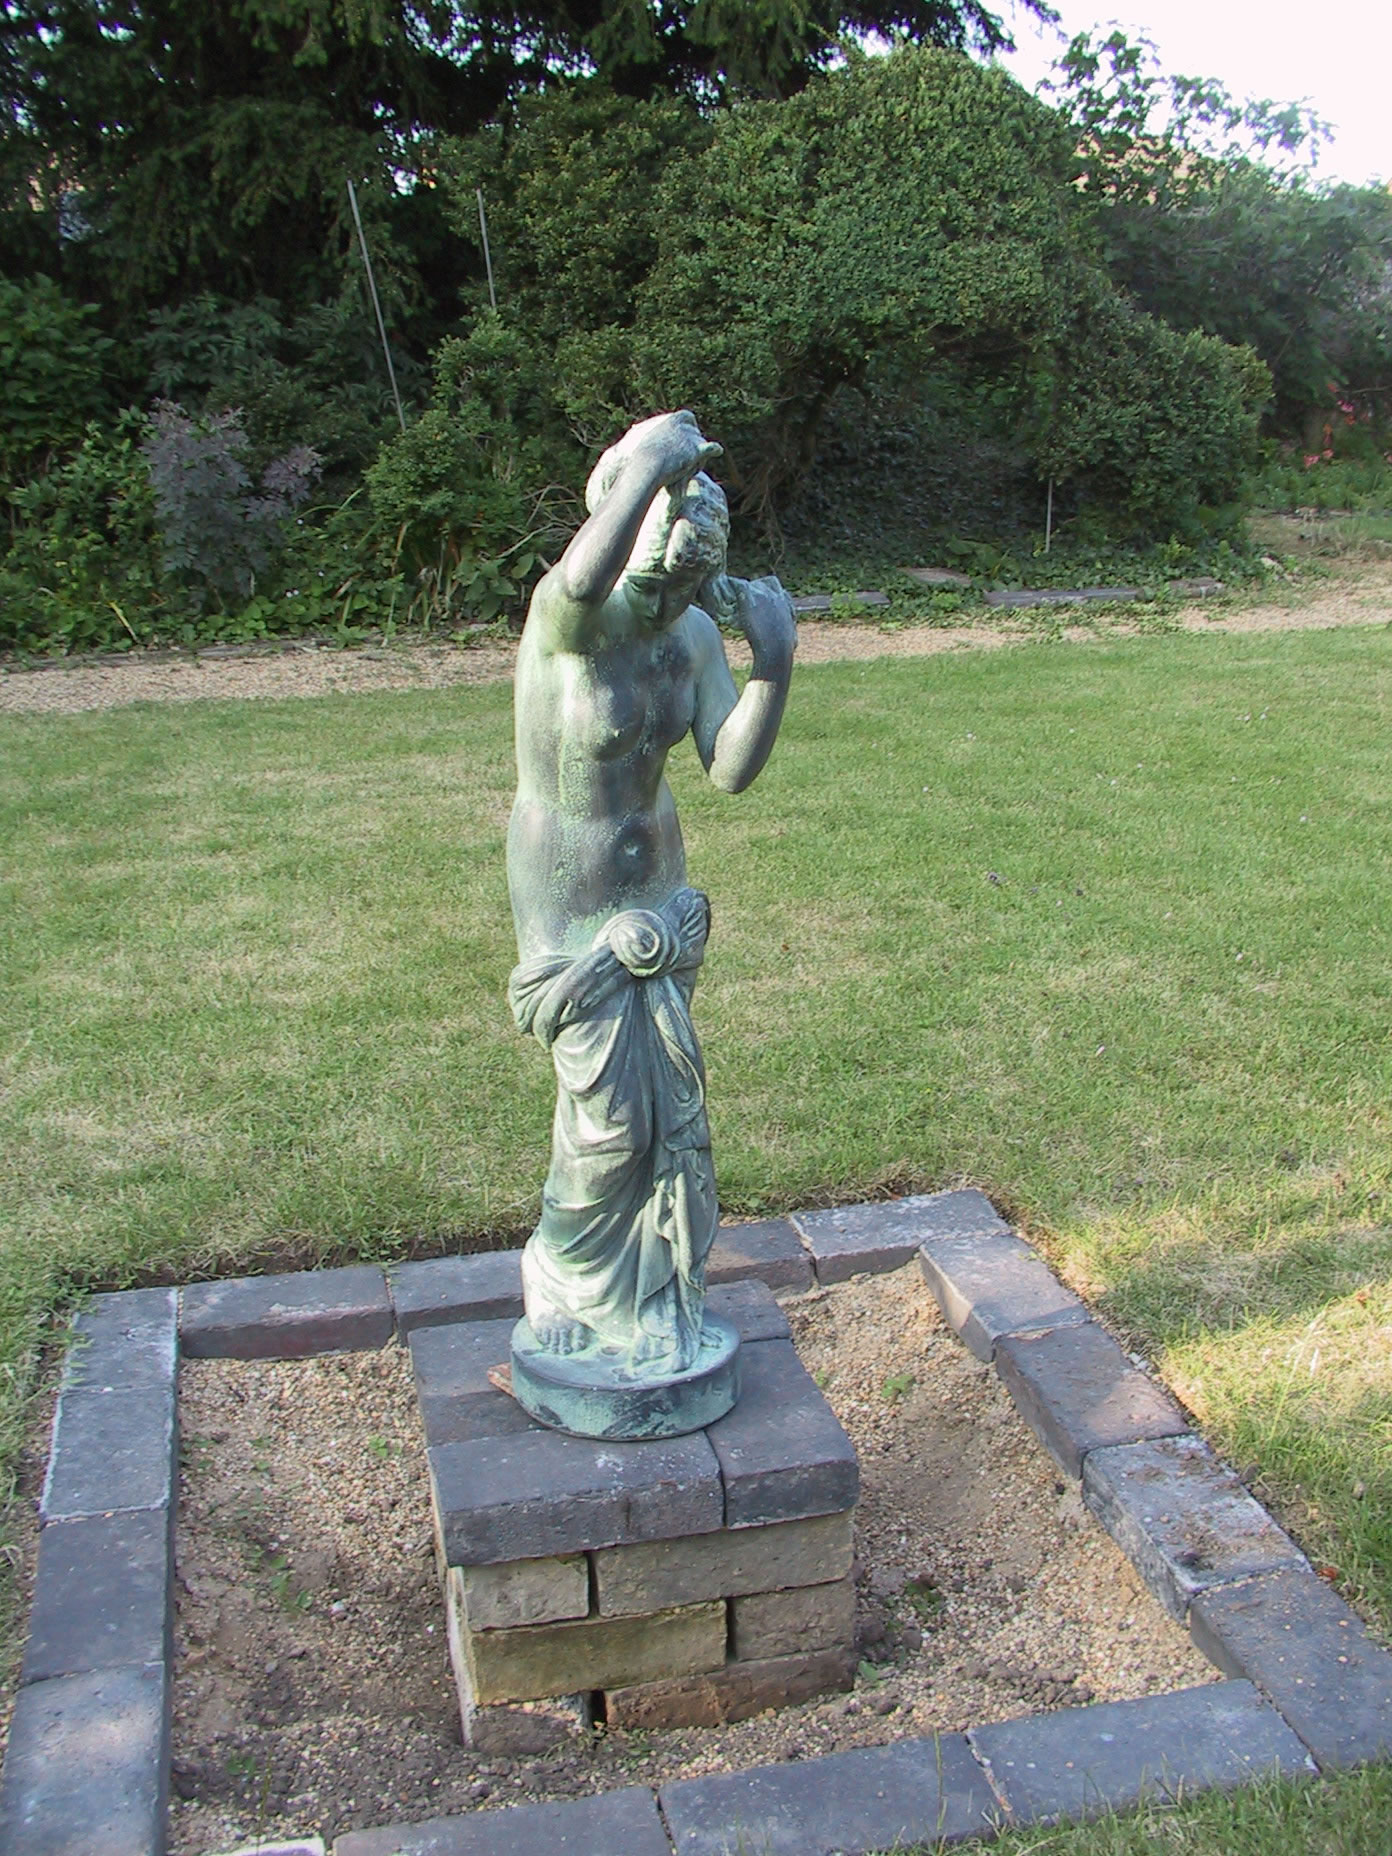
\includegraphics[height=0.3\textheight, width=0.6\textwidth]{statue.png}
            }
            \subfigure[output]{
                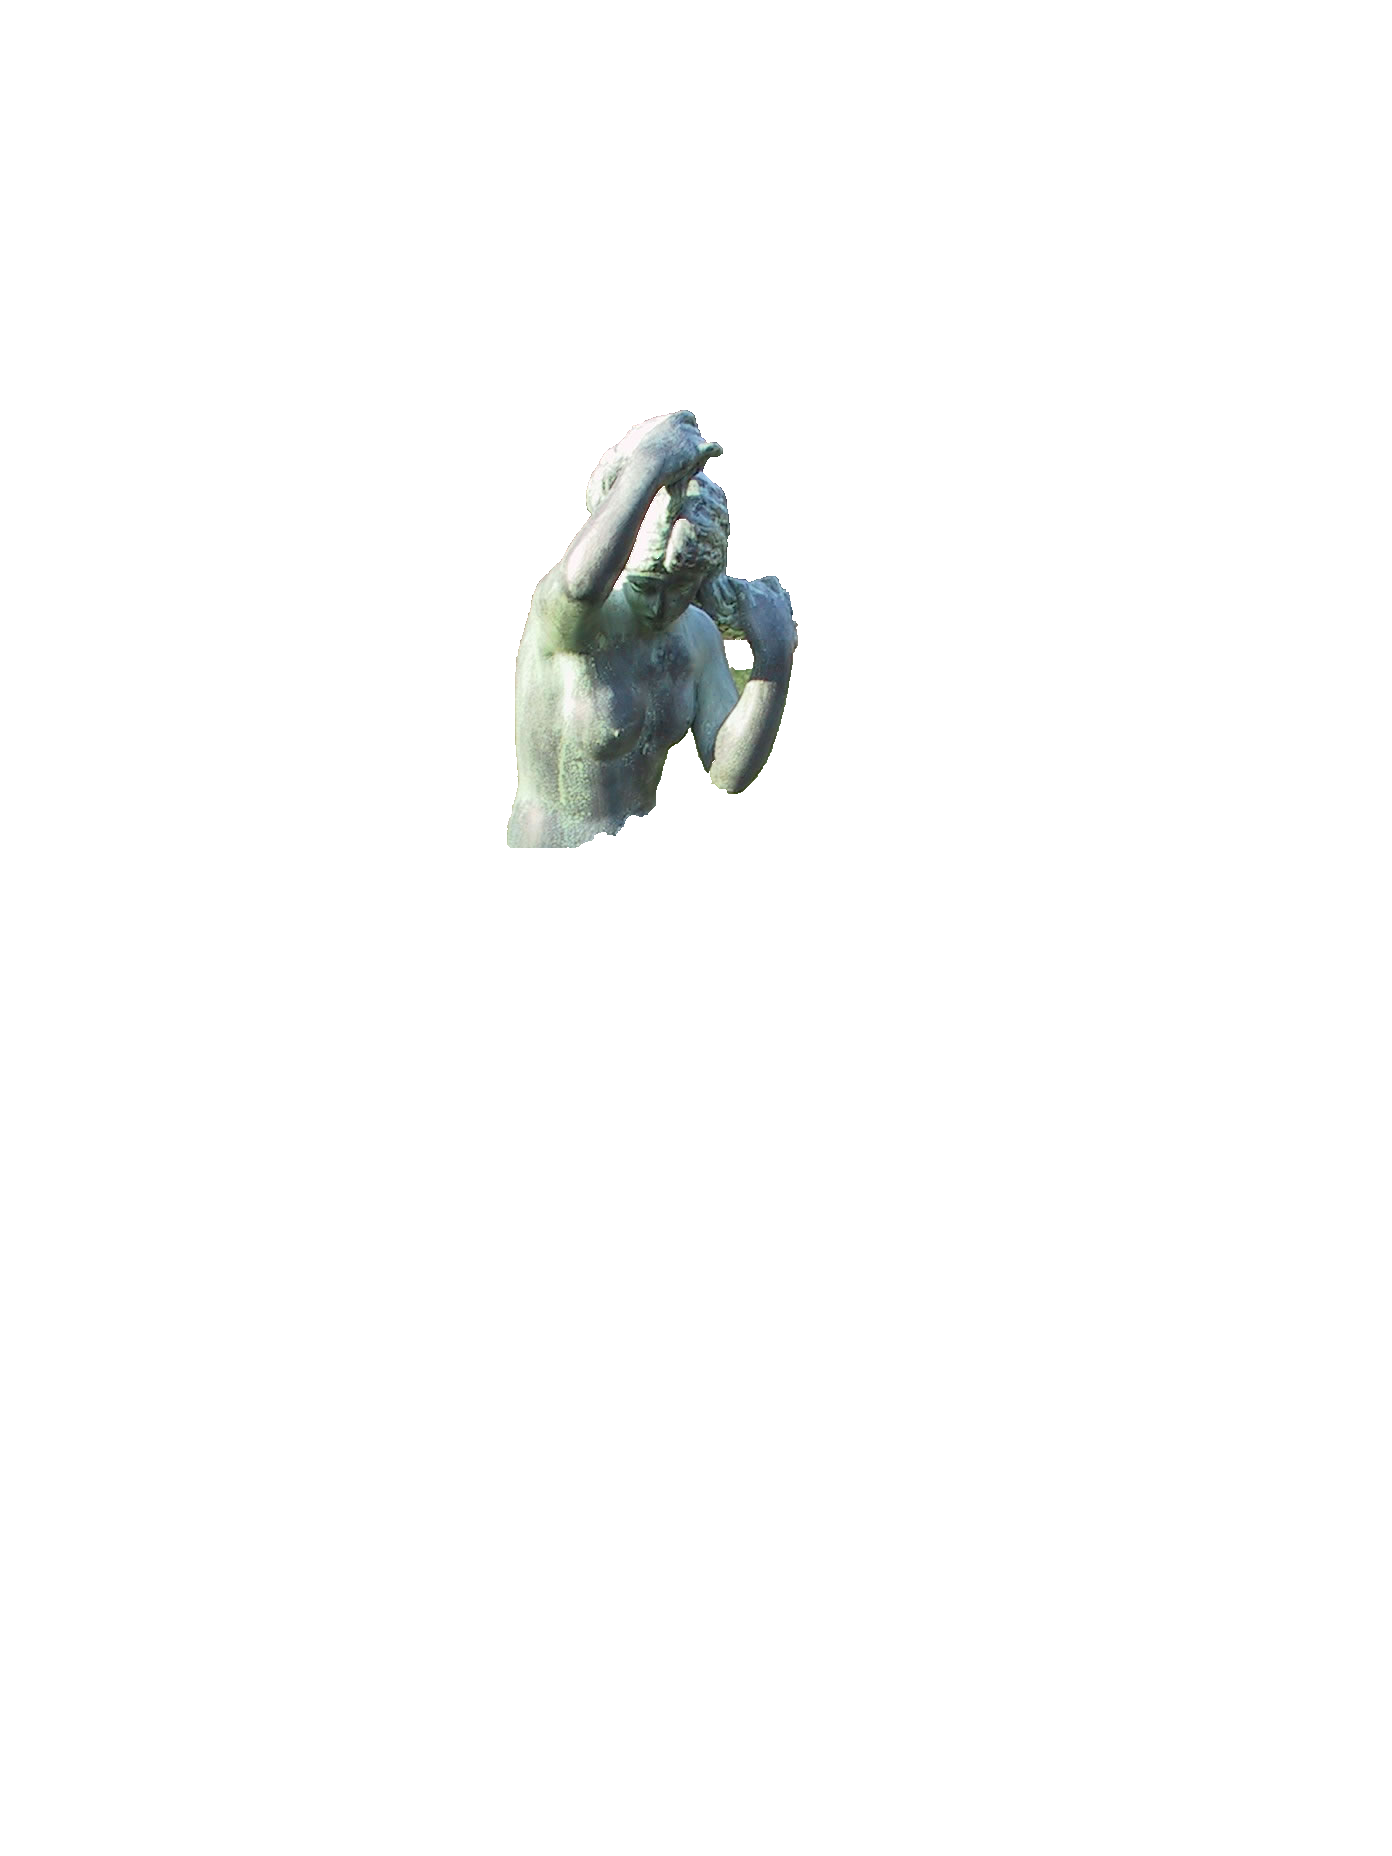
\includegraphics[height=0.3\textheight, width=0.6\textwidth]{output_statue.png}
            }
        \end{center}
        \caption{Statue}
    \end{figure}

    \begin{table}[!hbp]
        \begin{tabular}{|c|c|c|}
        \hline
        \hline
        Iteration & My Time(ms) & OpenCV Time(ms) \\
        \hline
        1 & 4004 & 4426 \\
        \hline
        2 &4855 & 5710 \\
        \hline
        5 & 8189 & 10260 \\
        \hline
        10 & 15442 & 20084 \\
        \hline
        \end{tabular}
        \caption{Comparsion with OpenCV}
    \end{table}

\renewcommand\refname{Reference}
\bibliographystyle{plain}
\bibliography{doc}

\end{document}